% Auf ungerader Seite starten
\cleardoublepage
%%%%%%%%%%%%%%%%%%%%%%%%%%%%%%%%%%%%%%%%%%%%%%%%%%%%%%%%%%%%%%%%%%%%%%%%%%%%%%%%%%%%%%%%%
% Zielsetzung und Vorgehensweise
%%%%%%%%%%%%%%%%%%%%%%%%%%%%%%%%%%%%%%%%%%%%%%%%%%%%%%%%%%%%%%%%%%%%%%%%%%%%%%%%%%%%%%%%%

\chapter{Weitere Hinweise}
\label{CHAPTER:Hinweise}

In diesem Kapitel wird auf einzelne Aspekte im Detail eingegangen. Zunächst wird die sprachliche Gestaltung behandelt, im weiteren Verlauf der Aufbau der Gliederung. Schließlich werden einige Besonderheiten zu Diagrammen, Abbildungen sowie Gleichungen erläutert.
\section{Sprachliche Gestaltung}
\label{SECTION:Sprache}

Das Ziel einer Abschlussarbeit ist, den untersuchten Sachverhalt möglichst einfach und leicht verständlich darzustellen. Komplizierte Satz- bzw. Wortstrukturen, die den Leser beeindrucken sollen, haben hier nichts zu suchen. Es ist sprachlich zwischen Gegenständen, beobachtbaren physikalischen Phänomenen, messbaren physikalische Größen und dem Wert der physikalischen Größen zu unterscheiden. Eine korrekte Formulierung ist beispielsweise: 
\begin{quote}
	\glqq Es findet Wärmeübertragung vom Fluid auf die Rohrleitung statt. Die Leitung ändert daher ihre Temperatur. Diese beträgt \SI{815}{\celsius}\grqq.
\end{quote}

Falsch ist hingegen: 

\begin{quote}
	\glqq Die Leitung hat \SI{815}{\celsius}\grqq~oder \glqq Die Wärmeübertragung wurde gemessen\grqq~und niemals: \glqq Die Leitung wurde gemessen\grqq.
\end{quote}

Ein Gegenstand hat genau einen Namen. Synonyme sind zu vermeiden, falls nicht völlig klar ist, dass mit beiden Begriffen dasselbe gemeint ist. Es sind aussagekräftige und eindeutige Beschreibungen zu verwenden. Zum Beispiel können Begriffe wie stromauf oder stromab eine eindeutigere Beschreibung liefern als horizontal oder vertikal. Auch rechts oder links sowie oben oder unten werden besser durch funktionsbezogene Lagebezeichnungen ersetzt. Beispielsweise: 

\begin{quote}
	\glqq Der Wirbel befindet sich stromab der rückspringenden Stufe im Strömungskanal. Zur Messung des Geschwindigkeitsfeldes im Wirbel wird eine Sonde quer zur Strömungsrichtung traversiert.\grqq
\end{quote}

Sätze, die sich über mehr als drei Zeilen erstrecken, stören den Lesefluss und werden besser in einzelne Sätze unterteilt. Zur Strukturierung von Sätzen zu Gedanken können Absätze eingesetzt werden. Sätze werden im Passiv konstruiert (kein \glqq man\grqq, \glqq ich\grqq, \glqq wir\grqq). Füllwörter, wie z.B. \glqq jedoch, hierfür, ...\grqq, sind zu vermeiden. Diese beinhalten keine Information und sind daher nicht notwendig. Lange Listen oder Aufzählungen sind ebenfalls zu vermeiden.

Eine korrekte Rechtschreibung und Interpunktion ist verpflichtend (Rechtschreibreform vom August 2006). Daher immer ein Rechtschreibprogramm nutzen! Als Dezimaltrennzeichen wird das Komma verwendet (\SI{1,3} {\km}). Bis auf Vorgehensweise und Zusammenfassung werden alle Kapitel im Präsens verfasst.

\section{Gliederung}
\label{SECTION:Gliederung}

\subsection{überflüssige Überschrift}

Auf einen Punkt x.y.1. folgt immer ein Punkt x.y.2. Wenn nicht, so ist der Punkt x.y.1 unnötig. Die Untergliederung auf der nächst höheren Ebene ist dann ausreichend. Empfehlung: Nach einer Kapitel- (Abschnitts-)Überschrift folgt i.d.R. Text und nicht etwa eine weitere Überschrift oder eine Abbildung. Gliedert sich das Kapitel X in X.1 und X.2, so könnte zu Beginn das Kapitels X z.B. stehen, was im Kap. X besprochen werden soll und wie sich dies auf die Unterkapitel aufteilt, warum die Themen des Kapitels X wichtig sind oder/und wie diese Themen mit dem Rest der Arbeit zusammenhängen. Die Gliederung ist so zu strukturieren, dass sie nicht mehr als drei Unterebenen (3.2.1, 3.2.1.1) enthält, vor allem nicht im Inhaltsverzeichnis. Treffende Überschriften wählen. Nicht \glqq Messaufbau\grqq, sondern \glqq Laseroptische Methode zur Untersuchung des Streuverhaltens\grqq.


\section{Literaturverweise}
\label{SECTION:Literaturverweise}

Alle zur Durchführung der Arbeit und zu deren Nutzen herangezogenen Quellen sind im Text zu beschreiben oder zumindest zu erwähnen und in einem Literaturverzeichnis am Ende des Hauptdokumentes aufzulisten. Außerdem sollten sie dem Betreuer in einer geeigneten Form verfügbar gemacht werden. Ist eine Quelle nur schwierig oder kurz verfügbar (z.B. weil ein Buch nur für kurze Zeit ausgeliehen werden darf), so ist eine Kopie der für die Arbeit wesentlichen Passagen anzufertigen. Internetquellen (auch Wikipedia) sind nicht als seriöse Quelle geeignet und mit adäquaten Fachliteraturquellen zu ersetzen. Falls die Angabe im Ausnahmefall notwendig ist, wird die Quelle in Form einer html-Datei oder eines Screenshots festgehalten. Direkte Zitate der Form:
\begin{quote}
	„In modernen Hochleistungstriebwerken betragen die Kühlluftmassenströme bereits über 30\% des gesamten Massenstroms der Kernmaschine.“ (\cite{baldauf2001}),
\end{quote}


sind zu vermeiden.

\nocite{*} % Alle Quellen werden im Quellenverzeichnis genannt, auch wenn Sie im Text nicht referenziert werden.

% Die folgenden Befehle helfen den Zitierstil gegebenenfalls anzupassen:
%\begin{tabbing}
%	\cite{baldauf2001,kneer2015}\\
%	\citep[s.a.][]{baldauf2001,kneer2015}\\
%	\citet{baldauf2001,kneer2015}\\
%	\\
%	\cite{winklhofer91,kneer2015}\\
%	\citep{winklhofer91,kneer2015}\\
%	\citet{winklhofer91,kneer2015}\\
%	\\
%	\cite{kneer2015}\\
%	\citep{kneer2015}\\
%	\citet{kneer2015}\\
%	\citet*{kneer2015}\\
%	\citeauthor{kneer2015}\\
%	\citeauthor*{kneer2015}\\
%	\citeyear{kneer2015}\\
%	\citeyearpar{kneer2015}\\
%	\\
%	\cite{winklhofer91}\\
%	\citep{winklhofer91}\\
%	\citet{winklhofer91}\\
%	\citet*{winklhofer91}\\
%	\citeauthor{winklhofer91}\\
%	\citeauthor*{winklhofer91}\\
%	\citeyear{winklhofer91}\\
%	\citeyearpar{winklhofer91}\\
%\end{tabbing}

\section{Abbildungen und Tabellen}
\label{SECTION:Abbildungen}

Abbildungen werden im Text erläutert: Abbildung~\ref{GRAPHIC:DomainKeller} lassen sich die physikalischen und geometrischen Eigenschaften des berechneten Gebiets entnehmen. Daher ist die Abbildung so platziert, dass sie nach dem Text erscheint, in dem diese beschrieben werden. Ebenso wird die Aussage der Abbildung erläutert: Die Fluid begrenzenden Flächen sind blau dargestellt, ... . Passiv konstruieren: Nicht \glqq Das Bild 2.4 zeigt\grqq, sondern \glqq In Bild 2.4 ist gezeigt\grqq. 

%Diese Abbildung wurde mit Inkscape erstellt, sodass die Grafik als pdf vorliegt, der Text aber in einer tex-Datei.

\begin{figure}[h]
	\centering
	\def\svgwidth{0.6\columnwidth}
	%\input{bilder/keller_2016.pdf_tex}	
	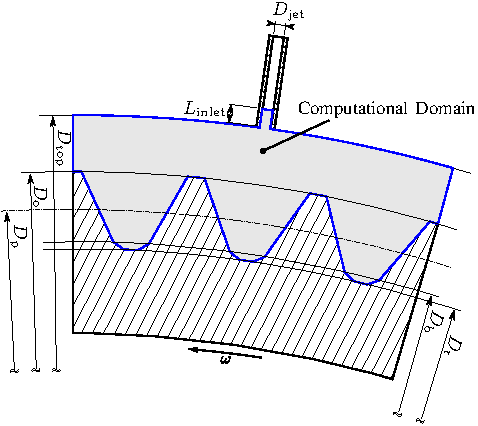
\includegraphics[width=0.7\textwidth]{bilder/keller_2016.pdf}
	\caption{Querschnitt durch das berechnete Segment des Zahnrads, \cite{keller2016}}
	\label{GRAPHIC:DomainKeller}
\end{figure}

% Die Platzierung der Abbildungen in figure-Umgebung kann anhand Optionen gesteuert werden:
% h - Die Abbildung wird wenn möglich an der Stelle der Definition eingefügt
% t - Die Abbildung wird oben auf der Seite platziert
% b - Die Abbildung wird unten auf der Seite platziert
% p - Eine eigene Seite mit Abbildungen wird angelegt
% Die Angabe von \begin{figure}[htbp] gibt die Priorität an. Zuerst wird versucht die Grafik an Ort und Stelle zu erzeugen. Gelingt dies nicht wird sie oben auf der Seite eingefügt, usw.

% Per \subcaptionbox können Abbildungen nebeneinander platziert und mit a), b) beschriftet werden
%\begin{figure}[ht]
%	\centering
%	\subcaptionbox{}{\includegraphics[width=0.48\columnwidth]{bilder/Bild_1_von_2}}\hfill
%	\subcaptionbox{}{\includegraphics[width=0.48\columnwidth]{bilder/Bild_2_von_2}}
%	\caption{GRAPHICS PLACED SIDE BY SIDE AND AMONG EACH OTHER WITH SUBORDINATE CAPTIONS}
%	\label{figure:_several_graphics}
%\end{figure}

Abbildungen helfen dem Autor, seine Erkenntnisse zu erläutern oder zu belegen. Diese Verbindung zwischen Abbildung und Aussage muss deutlich werden, sonst ist die Abbildung zu streichen. Alle Grafiken, Abbildungen und Tabellen müssen im Text referenziert und besprochen werden. Die Referenz ist durch eine fortlaufende Nummerierung der Objekte eindeutig vorzunehmen. Dabei werden Objekte gleichen Typs wie z.B. Abbildungen, Gleichungen und Tabellen jeweils gesondert nummeriert. Auf ein einheitliches Erscheinungsbild und Lesbarkeit achten (Textgröße, Auflösung, Größe angepasst an DIN A4, Vektorgrafiken wenn möglich). Abbildungen, die nicht selbst erstellt wurden, müssen ebenfalls zitiert werden. Wenn sie verändert wurden: \glqq Abbildung nach \cite{schoof2014}\grqq. Im Gegensatz zu Abbildungen besitzen Tabellen keine Unter- sondern Überschriften (siehe Tabelle \ref{tab:experiment-parameters}). Die Unterschriften sind möglichst aussagekräftig und eindeutig zu gestalten. Weitere Tabellenbeispiele werden von Markus Püschel\footnote{\url{https://www.inf.ethz.ch/personal/markusp/teaching/guides/guide-tables.pdf}} aufgezeigt. 

% Simple Beispiel-Tabelle
%\begin{table}[h]
%	\centering
%	\captionabove{Eine sinnlose Tabelle}
%	\begin{tabular}{|c|c|c|}
%		\hline
%		Spalte 1 & Spalte 2 & Spalte 3 \\
%		\hline
%		1 & 2 & 3 \\
%		\hlin den Diagrammen vergleichbar sein sollen (siehe Abbildung~\ref{fig:several_graphics}). Eventuell ist auch eine logarithmische Auftragung sinnvoll. Diagramme besitzen eine Legende. Sinnvolle min./max. Werte festlegen (nicht 0,2845 bis 9,385, sondern besser 0 bis 10). Ein Raster (\glqq grid\grqq) kann hilfreich sein. Diagramme farblich so gestalten, dass sie auch in schwarzweiß lesbar sind. In Abbildung \ref{fig:several_graphics} sind neben der farblichen Gestaltung zusätzlich unterschiedliche Marker und Linienarten eingesetzt. In der Regel ist der Hintergrund weiß, Sonderformatierungen (Hintergründe, Schriftarten) sind nur einzusetzen, wenn Vorteile daraus entstehen. Bei der Farbgebung auf die Erscheinungsform achten, zum Beispiel unterscheidet sich die Darstellung auf dem Beamer von der einer schriftlichen Ausarbeitung. Diagramme besitzen keinen alles umschließenden Rahmen. Abbildung möglichst einfach und leicht verständlich gestalten, in der Regel nicht mehr als drei Linien im Diagramm.

\begin{figure}[htpb]
	\centering
	\subcaptionbox{$x = \SI{0,7}{\mm}$} {\includeraphics[width=0.48\columnwidth]{bilder/wieth_2016_2_6}}\hfill
	\subcaptionbox{$x = \SI{1,0}{\mm}$}{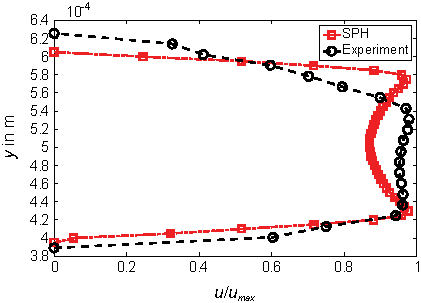
\includegraphics[width=0.48\columnwidth]{bilder/wieth_2016_2_6}}
	\subcaptionbox{$x = \SI{1,1}{\mm}$} {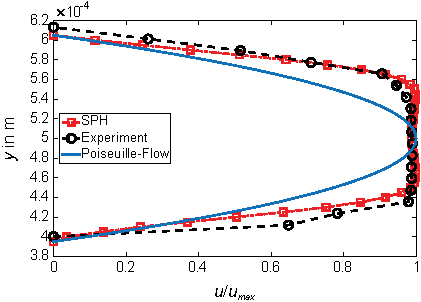
\includegraphics[width=0.48\columnwidth]{bilder/wieth_2016_3_6}}\hfill
	\subcaptionbox{$x = \SI{2.0}{\mm}$}{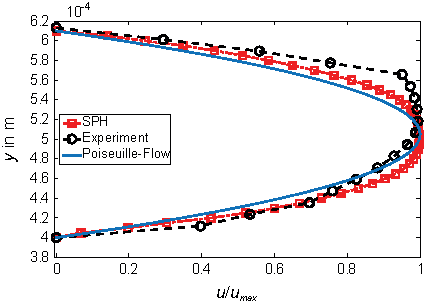
\includegraphics[width=0.48\columnwidth]{bilder/wieth_2016_4_6}}
	\subcaptionbox{$x = \SI{2,5}{\mm}$} {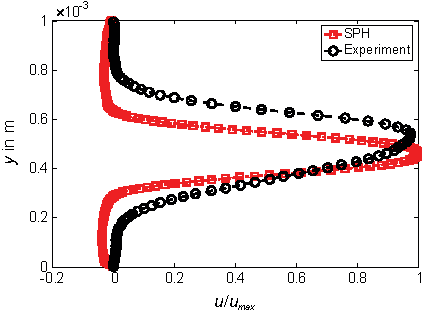
\includegraphics[width=0.48\columnwidth,height=5.5cm]{bilder/wieth_2016_5_6}}\hfill
	\subcaptionbox{$x = \SI{3,0}{\mm}$}{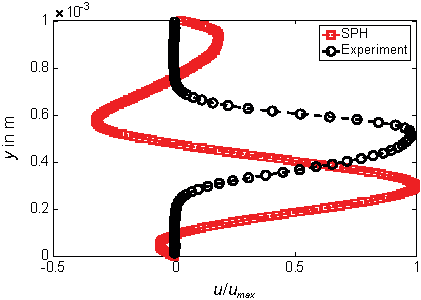
\includegraphics[width=0.48\columnwidth, height=5.5cm]{bilder/wieth_2016_6_6}}
	\caption{Vergleich zwischen experimentellen (kreisförmig) und berechneten (quadratisch) Werten, modifiziert nach \cite{wieth2016}. Da die Diagramme aus einer englischen Veröffentlichung stammen, sind die Dezimaltrennzeichen fälschlicherweise Punkte}
	\label{fig:several_graphics}
\end{figure}

\clearpage

\section{Gleichungen}
\label{SECTION:Gleichungen}

Alle Formelzeichen, die in einer Gleichung auftreten und nicht schon im vorangehenden Text definiert wurden, sind zu benennen und zu erläutern. In der Literatur etablierte Formelzeichen zur Beschreibung von physikalischen Größen wählen. Ein Formelzeichen beschreibt genau eine physikalische Größe. Jede physikalische Größe wird mit genau einem Formelzeichen beschrieben. Der Übersichtlichkeit halber mit Indizes und eingängigen Namen arbeiten. Gleichungen werden zentriert, nummeriert und sind Teil eines Satzes (besitzen also Satzzeichen). Zum Beispiel beschreibt der Impulssatz der Strömungsmechanik,

\begin{equation}
\label{EQUATION:Impuls}
\sum\vec{F}=\frac{d\vec{I}}{dt}=\underbrace{\frac{\partial}{\partial t}\iiint\varrho\:\vec{w}\:dV}_{\text{instationär}} + \underbrace{\iint\varrho\:\vec{w}\:\left(\vec{w}\cdot\vec{n}\right)\:dA}_{\text{stationär}},
\end{equation}

die zeitliche Änderung des Impulses $\frac{d\vec{I}}{dt}$ innerhalb eines Kontrollvolumens $V$, mit  der Dichte $\varrho$, dem Geschwindigkeitsvektor $\vec{w}$, der Oberfläche $A$ und dem äußeren Oberflächennormalen-Einheitsvektor $\vec{n}$. Die Änderung des Impulses entspricht der Summe der äußeren Kräfte $\sum\vec{F}$.

Formelzeichen werden immer zusammen mit einer Bezeichnung erwähnt. Die Angabe des Werts einer physikalischen Größe erfolgt immer mit der entsprechenden Einheit:

\begin{quote}
	$\Delta T$ = \SI{452,69}{\kelvin}.
\end{quote}

Zwischen Größe und Einheit, wie \SI{2,0}{\mm}, wird ein halbes Leerzeichen gesetzt (umbruchgeschütztes Leerzeichen verwenden bzw. \LaTeX-Paket siunitx). Einheiten und Operatoren, wie \glqq log\grqq, werden nicht kursiv gesetzt. Innerhalb der Arbeit auf eine einheitliche Darstellung für Vektoren, Tensoren etc. achten und SI-Einheiten verwenden.

%Formeln über mehrere Zeilen können zum Beispiel so realisiert werden:
%\begin{eqnarray}
%\sigma_e & = & n_0 \pi r^2 \xi_e \nonumber \\
%\sigma_s & = & n_0 \pi r^2 \xi_s \\
%\sigma_a & = & \sigma_e - \sigma_a
%\end{eqnarray}
% & richtet die einzelnen Zeilen zueinander aus.

%\section {Some text}
%TeX does not mean only programing and using commands. Examining the source-code of the text below, you will realise that typing a bigger paragraph of text is relatively simple and does not require more effort for formatting than with other programs. In the text-section below, among other things, some examples for font formatting and referencing are given.
%
%Fig.~\ref{figure:_zeilenumbruch} shows selected results of the LDV measurements of the gaseous 
%phase. In the upper diagram the phase averaged temporal 
%variation of the vertical component (axial velocity) 
%$u_{G,Y}(\phi)=\overline{u}_{G,Y}+u'_{G,Y}(\phi)$ is presented for a pulsating gaseous flow at a constant excitation 
%frequency of $f_S=\SI{250}{Hz}$, different mean velocities $\overline{u}_G$ and a constant 
%bypass setting of the siren. Apparently, the instantaneous 
%velocity $u_{G,Y}(\phi)$ is increasing with the mean velocity $\overline{u}_G$. However, the 
%relation is not proportional. There is a loss of velocity due to the positioning of the 
%LDV measuring volume in the wake of the prefilming surface and the divergence of the open jet. 
%Furthermore, the phase shift 
%is moving towards an earlier time at higher mean velocities. This can be explained by 
%the longer wavelength $\lambda \approx \overline{u}_G/f_S$ of the convected pulsation.
%It has to be noted that the signals are not perfectly sinusoidal 
%as anticipated. The fundamental mode is superimposed by a 
%first and second harmonic oscillations and additional noise. However, 
%those perturbing components represent only a fraction of the 
%designated signal.
